\documentclass{beamer}
\usepackage{../../shared/styles/custom}
\usepackage{../../shared/styles/conventions}
\usepackage{comment}

\usepackage{multicol}
%\beamerdefaultoverlayspecification{<+->}


\makeatletter
\def\magicomadjust{0em}  % a way to adjust if the spacing should be different
\newdimen\indent@amount
\def\magicom{\relax
  \ifhmode $$%
    \predisplaypenalty\@M \postdisplaypenalty\@M
    \abovedisplayskip-\baselineskip \belowdisplayskip\z@
    \abovedisplayshortskip\abovedisplayskip
    \belowdisplayshortskip\belowdisplayskip
    \global\indent@amount\predisplaysize
     $$\count@\prevgraf \advance\count@-\thr@@
         \prevgraf\count@
    \global\advance\indent@amount-2em  % correction for \predisplaysize indent
    \global\advance\indent@amount\magicomadjust  % correction for verse env, for example
    \hspace*\indent@amount
  \else\typeout{*Not in hmode*}\fi}
\makeatother



\begin{comment}

	\ifx\relax#1\relax  \item \else \item[#1] \fi
	\abovedisplayskip=0pt\abovedisplayshortskip=0pt~\vspace*{-\baselineskip}}

\end{comment}


\title{Support Vector Machines}
\date{\today}
\author{Nipun Batra}
\institute{IIT Gandhinagar}

\begin{document}
\maketitle

\begin{frame}{Outline}
\tableofcontents
\end{frame}


\section{Introduction and Motivation}

{
	\setbeamercolor{background canvas}{bg=}
	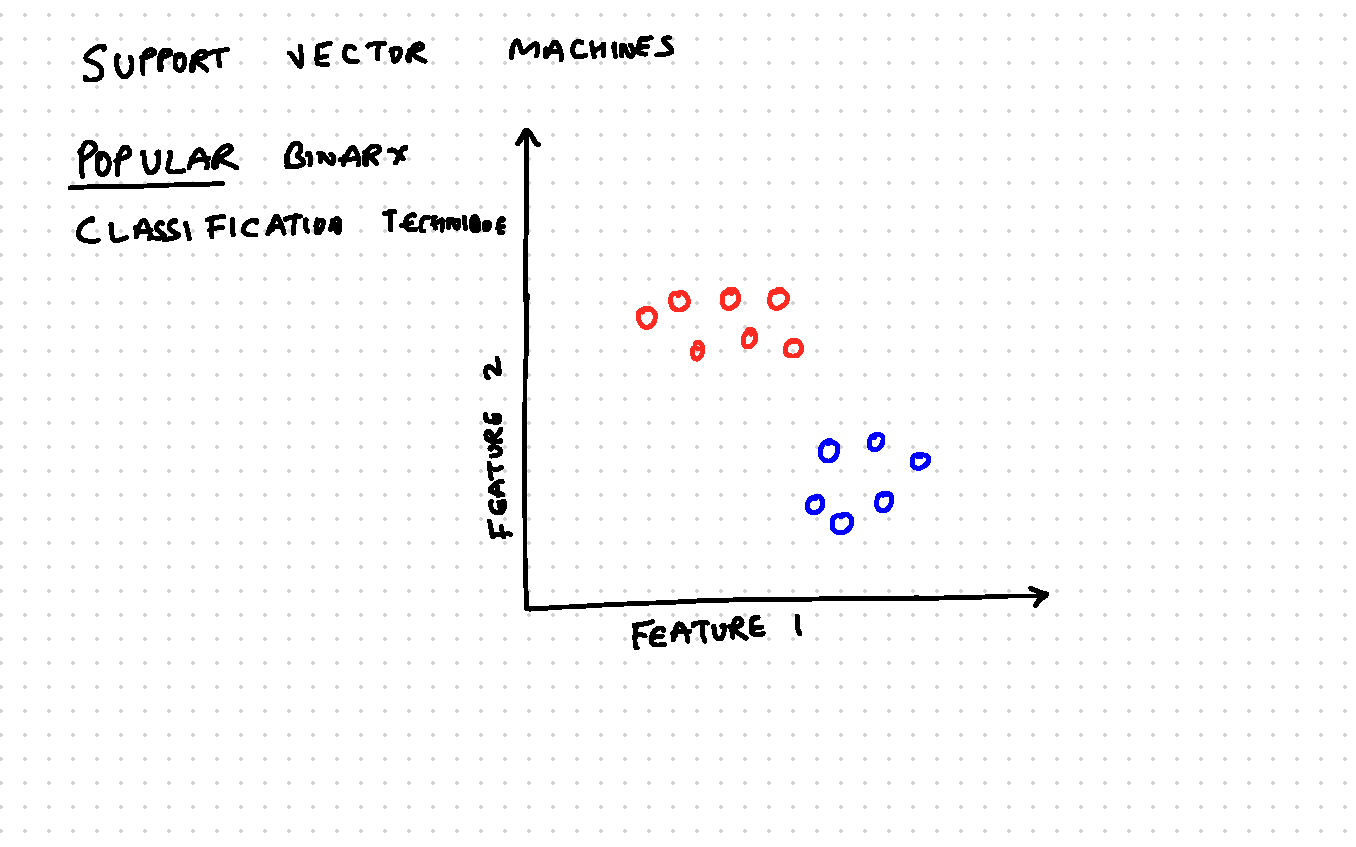
\includepdf[page=1-19]{../assets/svm/Svm-notes.pdf}
}

\section{Mathematical Foundation}

\begin{frame}{Distance between 2 parallel hyperplanes}
Equation of two planes is:
$$
\begin{aligned}
&\vw\cdot \vx+b_1=0\\
&\vw\cdot \vx+b_2=0
\end{aligned}
$$

\pause For a point $\vx_1$ on plane 1 and $\vx_2$ on plane 2, we have:
\pause $$
\begin{array}{l}
{\vx_{2}=\vx_{1}+t \vw} \\
{D=|t \vw|=|t|\|\vw\|}
\end{array}
$$

\pause We can rewrite as follows:
\pause $$
\begin{array}{c}
{\vw \cdot \vx_{2}+b_{2}=0} \\
{\Rightarrow \vw \cdot\left(\vx_{1}+t \vw\right)+b_{2}=0}
\end{array}
$$
\pause $$
\Rightarrow \vw \cdot \vx_{1}+t\|\vw\|^{2}+b_1-b_1+b_2 = 0
\Rightarrow t = \frac{b_1 - b_2}{\|\vw\|^{2}}  \Rightarrow D = t\|\vw\| =  \frac{|b_1 - b_2|}{\|\vw\|}
$$
\end{frame}

\begin{frame}{Pop Quiz \#1}
\begin{tcolorbox}[colback=blue!5!white,colframe=blue!75!black,title=Quick Question!]
If two parallel hyperplanes are given by:
\begin{itemize}
	\item $\vw \cdot \vx + 3 = 0$
	\item $\vw \cdot \vx - 1 = 0$
\end{itemize}
And $\|\vw\| = 2$, what is the distance between them?

\pause
\textbf{Answer:} $D = \frac{|3 - (-1)|}{2} = \frac{4}{2} = 2$ units
\end{tcolorbox}
\end{frame}

\section{SVM Formulation}

{
	\setbeamercolor{background canvas}{bg=}
	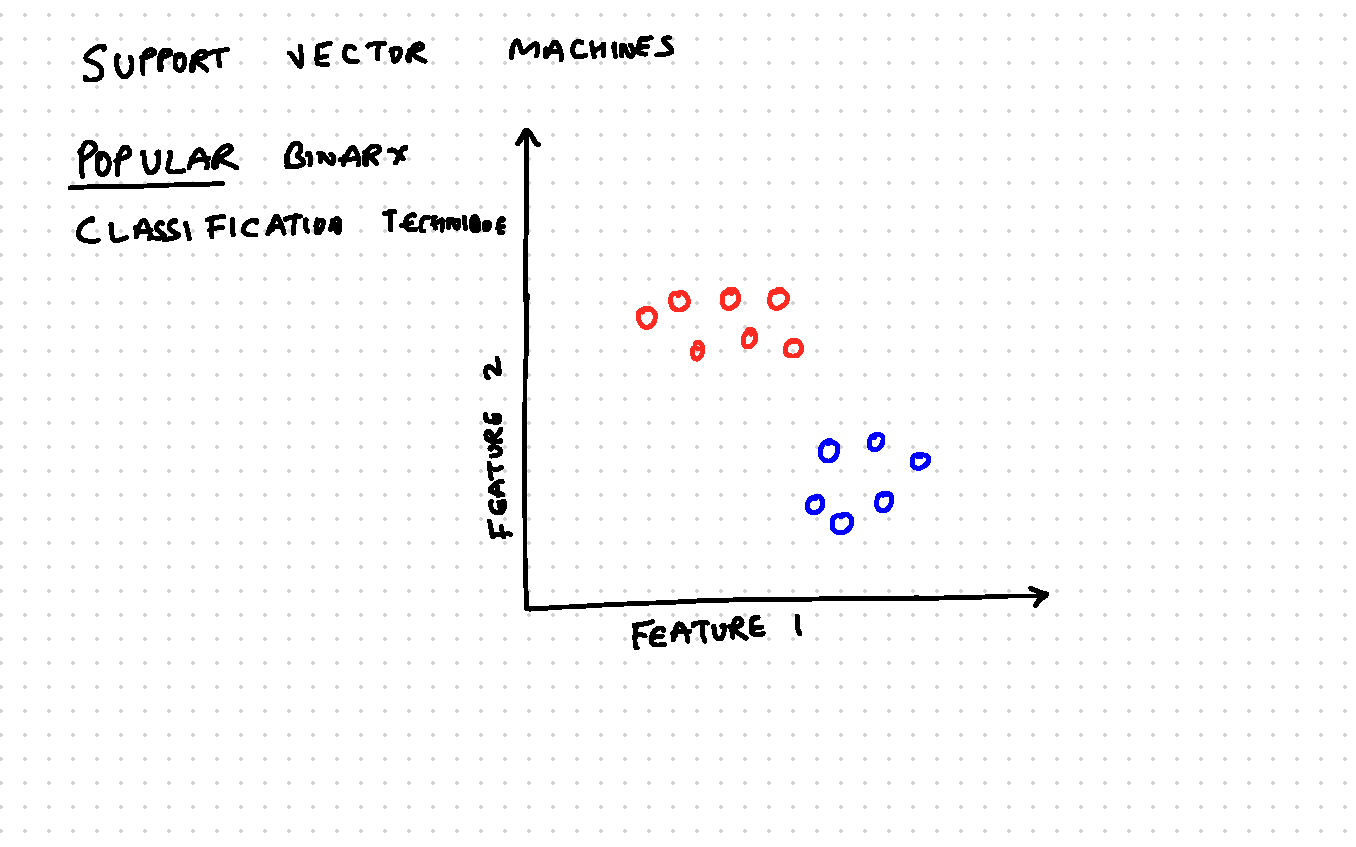
\includepdf[page=20-25]{../assets/svm/Svm-notes.pdf}
}

\begin{frame}{Primal Formulation}
	\begin{tcolorbox}{Objective}
	\begin{align*}
	\minimize & \frac{1}{2}\norm{\vw}^{2} \\
	\subjectto & y_{i}(\vw \cdot \vx_{i} + b) \geq 1 \quad \forall i
	\end{align*}
\end{tcolorbox}
\pause 
Q) What is $\norm{\vw}$?
\pause
\begin{multicols}{2}
\begin{equation*}
	 \vw = \begin{bmatrix}
	 w_{1} \\
     w_{2} \\
     \vdots  \\
     w_{n} \\
	\end{bmatrix}
\end{equation*}\break
\begin{align*}
	 \norm{\vw} &= \sqrt{\vw\tp\vw}\\
	 &= \sqrt{\begin{bmatrix}
	 w_{1} & w_{2} & \cdots & w_{n}
	 \end{bmatrix}
	 \begin{bmatrix}
	  w_{1} \\
	  w_{2} \\
     \vdots  \\
     w_{n} \\
	 \end{bmatrix}}
\end{align*}

\end{multicols}

\end{frame}

\section{Worked Example}

{
	\setbeamercolor{background canvas}{bg=}
	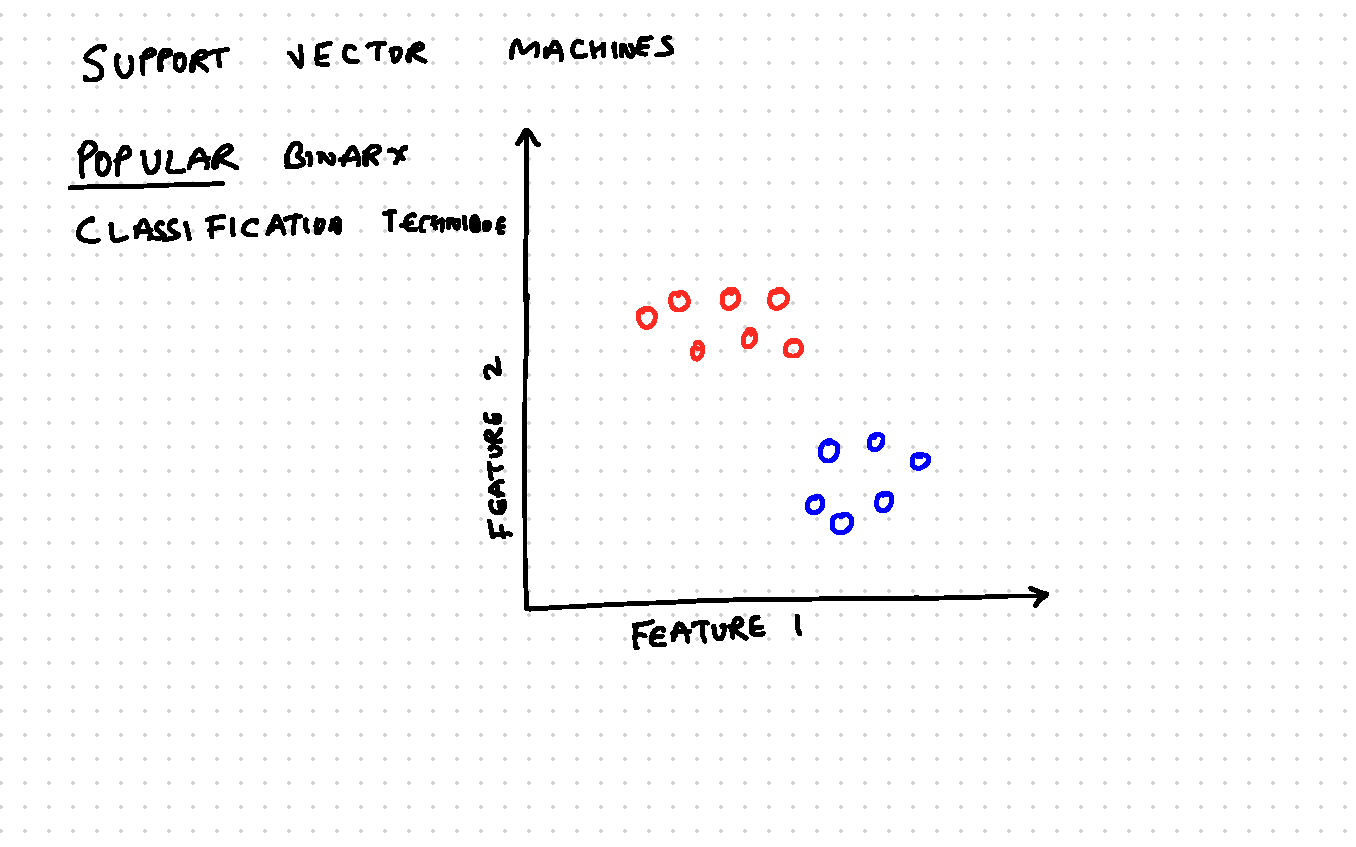
\includepdf[page=27]{../assets/svm/Svm-notes.pdf}
}

\begin{frame}{Simple Exercise}

\begin{align*}
\begin{bmatrix}
x && y \\
1 && 1\\
2 && 1\\
-1 && -1\\
-2 && -1\\
\end{bmatrix}
\end{align*}
Separating Hyperplane: $\vw \cdot \vx + b = 0$
\end{frame}

\begin{frame}{Simple Exercise}
\begin{tcolorbox}

\begin{equation*}
y_{i}(\vw \cdot \vx_{i} + b) \geq 1
\end{equation*}
\end{tcolorbox}
\begin{multicols}{2}
\begin{equation*}
\begin{bmatrix}
x_{1} && y \\
1 && 1\\
2 && 1\\
-1 && -1\\
-2 && -1\\
\end{bmatrix}
\end{equation*}\break

\begin{align*}
&\Rightarrow y_{i}(w \cdot x_{i} + b) \geq 1\\
&\Rightarrow 1(w \cdot 1 + b) \geq 1\\
&\Rightarrow 1(w \cdot 2 + b)\geq 1\\
&\Rightarrow -1(w \cdot (-1)+b) \geq 1\\
&\Rightarrow -1(w \cdot (-2)+b) \geq 1\\
\end{align*}


\end{multicols}
\end{frame}

{
	\setbeamercolor{background canvas}{bg=}
	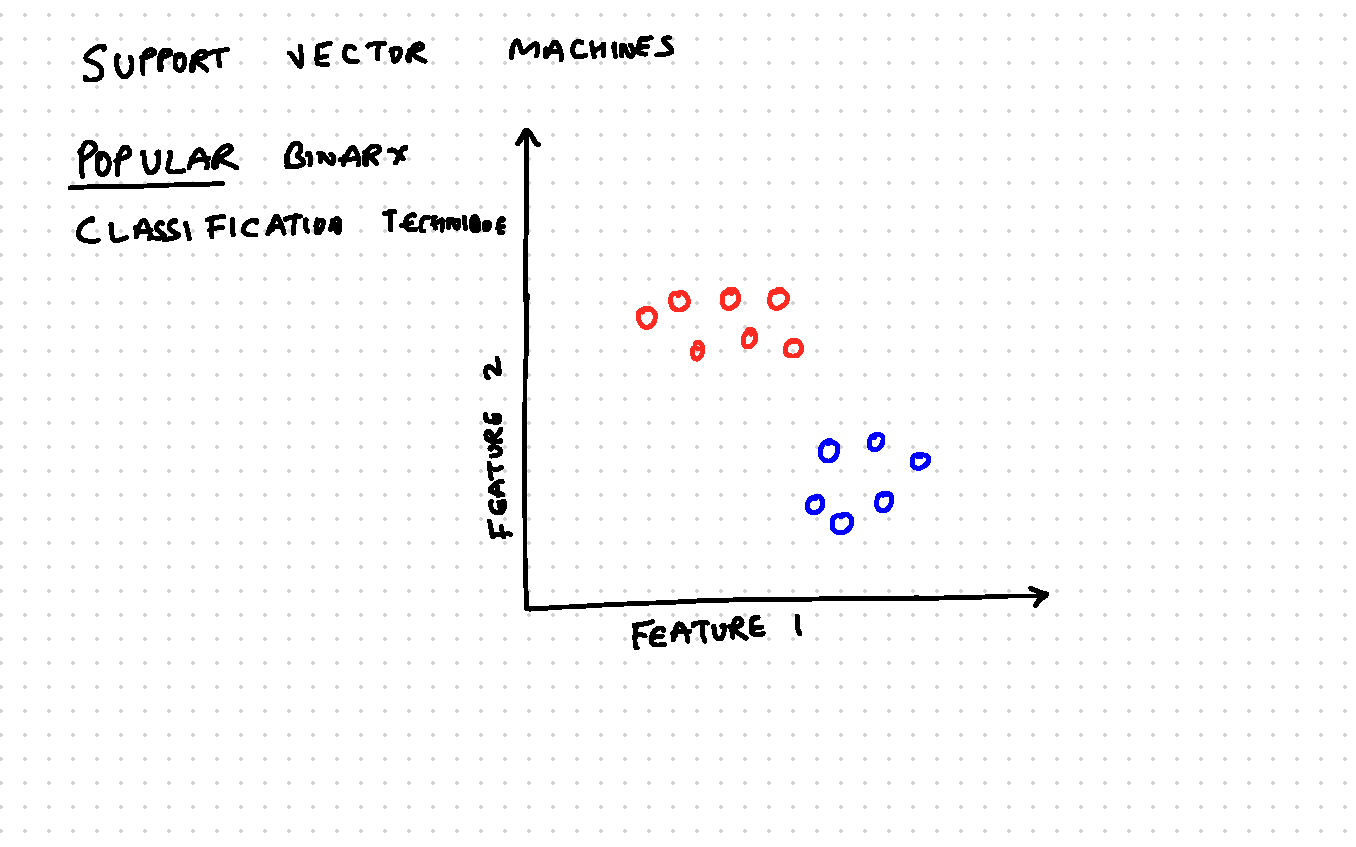
\includepdf[page=28-33]{../assets/svm/Svm-notes.pdf}
}


\begin{frame}{Simple Exercise}

\begin{align*}
w_{min} = 1, b&= 0\\
w.x + b &= 0\\
x &=0 \\
\end{align*}

\end{frame}

\begin{frame}{Simple Exercise}
Minimum values satisfying constraints  $\Rightarrow$
$w$ = 1 and $b = 0$\\
$\therefore$ Max margin classifier $ \Rightarrow x = 0$

\end{frame}

\begin{frame}{Pop Quiz \#2}
\begin{tcolorbox}[colback=blue!5!white,colframe=blue!75!black,title=Think About This!]
In our simple 1D example, why did we choose $w = 1$ and $b = 0$ as the optimal solution?

\pause
\begin{itemize}
	\item Is this the \textbf{only} solution that separates the data?
	\item What makes this solution \textbf{optimal} for SVM?
\end{itemize}

\pause
\textbf{Answer:} No, infinitely many solutions exist (e.g., $w = 2, b = 0$ or $w = 0.5, b = 0$). \\
SVM chooses $w = 1, b = 0$ because it minimizes $\|\vw\|^2$ while satisfying all constraints!
\end{tcolorbox}
\end{frame}

\begin{frame}{Primal Formulation is a Quadratic Program}
\begin{align*}
\text{Generally;}&\\
&\Rightarrow \text{Minimize Quadratic(x)}\\
&\Rightarrow \text{such that, Linear(x)}
\end{align*}
\begin{tcolorbox}
Question
\begin{align*}
&{x} = (x_{1}, x_{2})\\
&\text{minimize} \hspace{3mm} \frac{1}{2}||x||^{2}\\
&\colon x_{1} + x_{2} - 1 \geq 0
\end{align*}
\end{tcolorbox}
\end{frame}



{
	\setbeamercolor{background canvas}{bg=}
	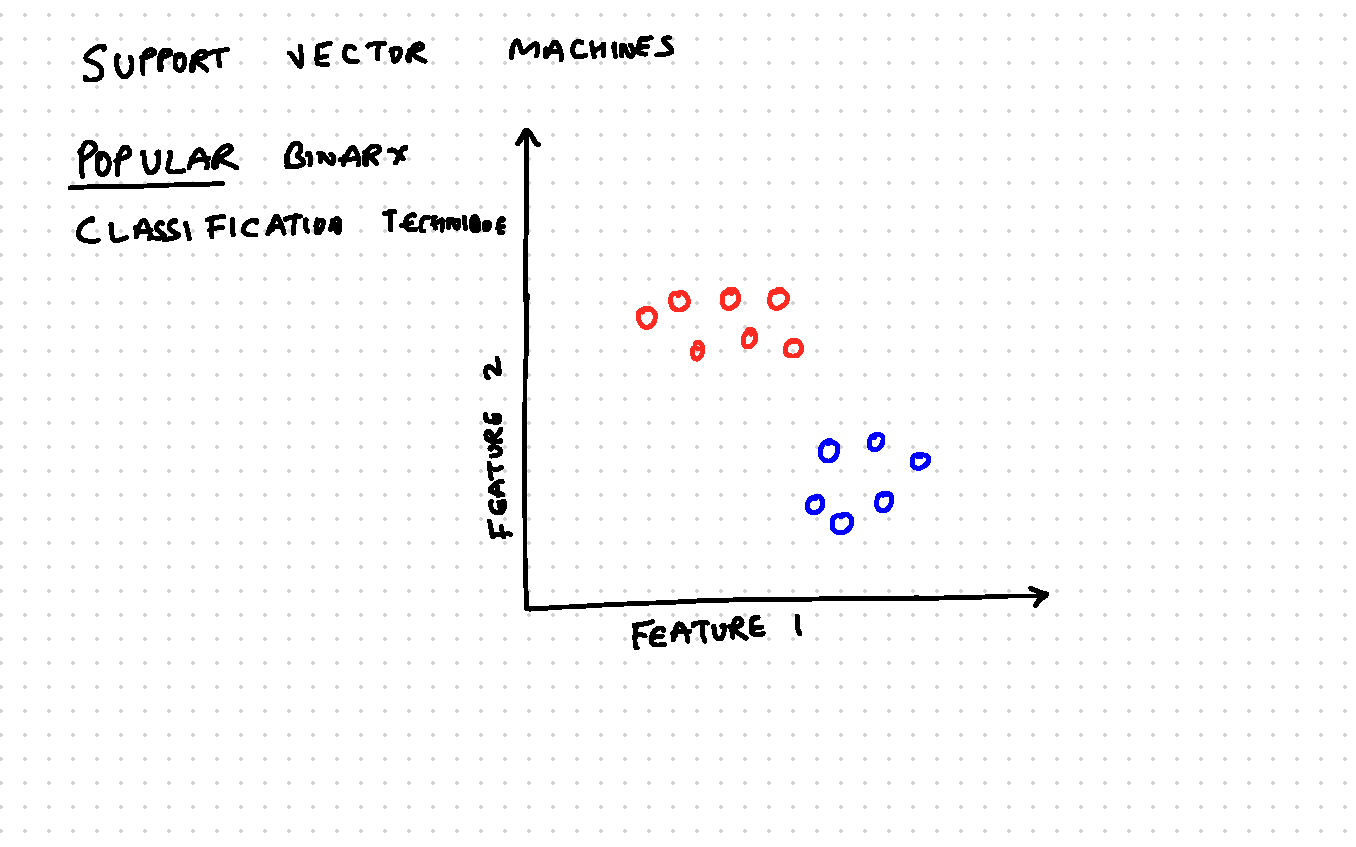
\includepdf[page=34]{../assets/svm/Svm-notes.pdf}
}



\begin{frame}{Converting to Dual Problem}
Primal $\Rightarrow$ Dual Conversion using Lagrangian multipliers\\
\begin{align*}
	\text{Minimize } & \frac{1}{2}\|\vw\|^{2} \\
	\text{s.t. } & y_{i}(\vw \cdot \vx_{i} + b) \geq 1\\
	 \hspace{2mm}\forall i
	\end{align*}
\begin{align*}
&L(\vw,b,\valpha) = \frac{1}{2}
\sum_{i = 1}^{d} w_{i}^{2} - \sum_{i=1}^{N} \alpha_{i}(y_{i}(\vw \cdot \vx_{i} + b) - 1) \hspace{2mm} \forall \hspace{2mm}\alpha_{i} \geq 0\\
&\frac{\partial L}{\partial b} = 0 \Rightarrow \sum_{i=1}^{n}\alpha_{i}y_{i} = 0\\
\end{align*}
\end{frame}

\begin{frame}{Converting to Dual Problem}
\begin{align*}
\frac{\partial L}{\partial \vw} = 0 \Rightarrow & \vw - \sum_{i=1}^{n}\alpha_{i}y_{i}\vx_{i} = 0\\
& \vw = \sum_{i=1}^{N}\alpha_{i}y_{i}\vx_{i}
\end{align*}
\begin{align*}
&L(\vw,b,\valpha) = \frac{1}{2}
\sum_{i = 1}^{d} w_{i}^{2} - \sum_{i=1}^{N} \alpha_{i}(y_{i}(\vw \cdot \vx_i + b) -1)\\
&= \frac{1}{2}\|\vw\|^{2}-\sum_{i=1}^{N} \alpha_{i} y_{i} \vw \cdot \vx_{i}-\sum_{i=1}^{N} \alpha_{i} y_{i} b+\sum_{i=1}^{N} \alpha_{i}\\
&= \sum_{i=1}^{N} \alpha_{i}+\frac{\left(\sum_{i} \alpha_{i} y_{i} \vx_{i}\right) \cdot \left(\sum_{j} \alpha_{j} y_{j} \vx_{j}\right)}{2}-\sum_{i} \alpha_{i} y_{i}\left(\sum_{j} \alpha_{j} y_{j} \vx_{j}\right) \cdot \vx_{i}
\end{align*}
\end{frame}

\begin{frame}{Converting to Dual Problem}
\begin{align*}
&L(\valpha)=\sum_{i=1}^{N} \alpha_{i}-\frac{1}{2} \sum_{i=1}^{N} \sum_{j=1}^{N} \alpha_{i} \alpha_{j} y_{i} y_{j} \vx_{i} \cdot \vx_{j}\\
\end{align*}
\begin{tcolorbox}
\begin{align*}
&\begin{array}{ll}
{\text { Minimize }\|\vw\|^{2} \Rightarrow}&{\text{Maximize } L(\valpha)} \\
{  s.t  } & {  s.t  } \\
{y_{i}\left(\vw \cdot \vx_{i}+b\right) \geqslant 1} & {\sum_{i=1}^{N} \alpha_{i} y_{i}=0 \hspace{2mm}\forall \hspace{2mm} \alpha_{i}  \geq 0}
\end{array}
\end{align*}
\end{tcolorbox}
\end{frame}

\begin{frame}{Pop Quiz \#3}
\begin{tcolorbox}[colback=blue!5!white,colframe=blue!75!black,title=Lagrangian Mystery!]
Why do we convert the primal SVM problem to its dual formulation?

\pause
\textbf{Hint:} Think about what the dual formulation enables us to do that the primal doesn't...

\pause
\textbf{Answer:} The dual formulation enables the \textbf{kernel trick}! 
\begin{itemize}
	\item Primal: $\vw$ appears explicitly $\rightarrow$ no kernels
	\item Dual: Only dot products $\vx_i \cdot \vx_j$ appear $\rightarrow$ can replace with $K(\vx_i, \vx_j)$
\end{itemize}
\end{tcolorbox}
\end{frame}

\begin{frame}{Question: KKT Complementary Slackness}
\textbf{Question}:\\
\vspace{2mm}
$\alpha_{i}\left(y_{i}\left(\vw \cdot \vx_{i}+b\right)-1\right)=0 \quad \forall i$ as per KKT slackness\\
\vspace{2mm}
What is $\alpha_{i}$ for support vector points?\\
\vspace{4mm}
\textbf{Answer:}
For support vectors,\\
\hspace{1in}$\vw \cdot \vx_{i} + b  = -1$ (for $y_i = -1$)\\
\hspace{1in}$\vw \cdot \vx_{i} + b  = +1$ (for $y_i = +1$)\\
\vspace{2mm}
$y_{i}\left(\vw \cdot \vx_{i}+b\right)-1=0 \quad \text {for } i \in \{\text{support vector points}\}$\\
$\therefore \alpha_{i} \neq 0$ where $i \in \{\text{support vector points}\}$
\vspace{5mm}
$\text{For all non-support vector points: }\alpha_{i} = 0$
\end{frame}

{
	\setbeamercolor{background canvas}{bg=}
	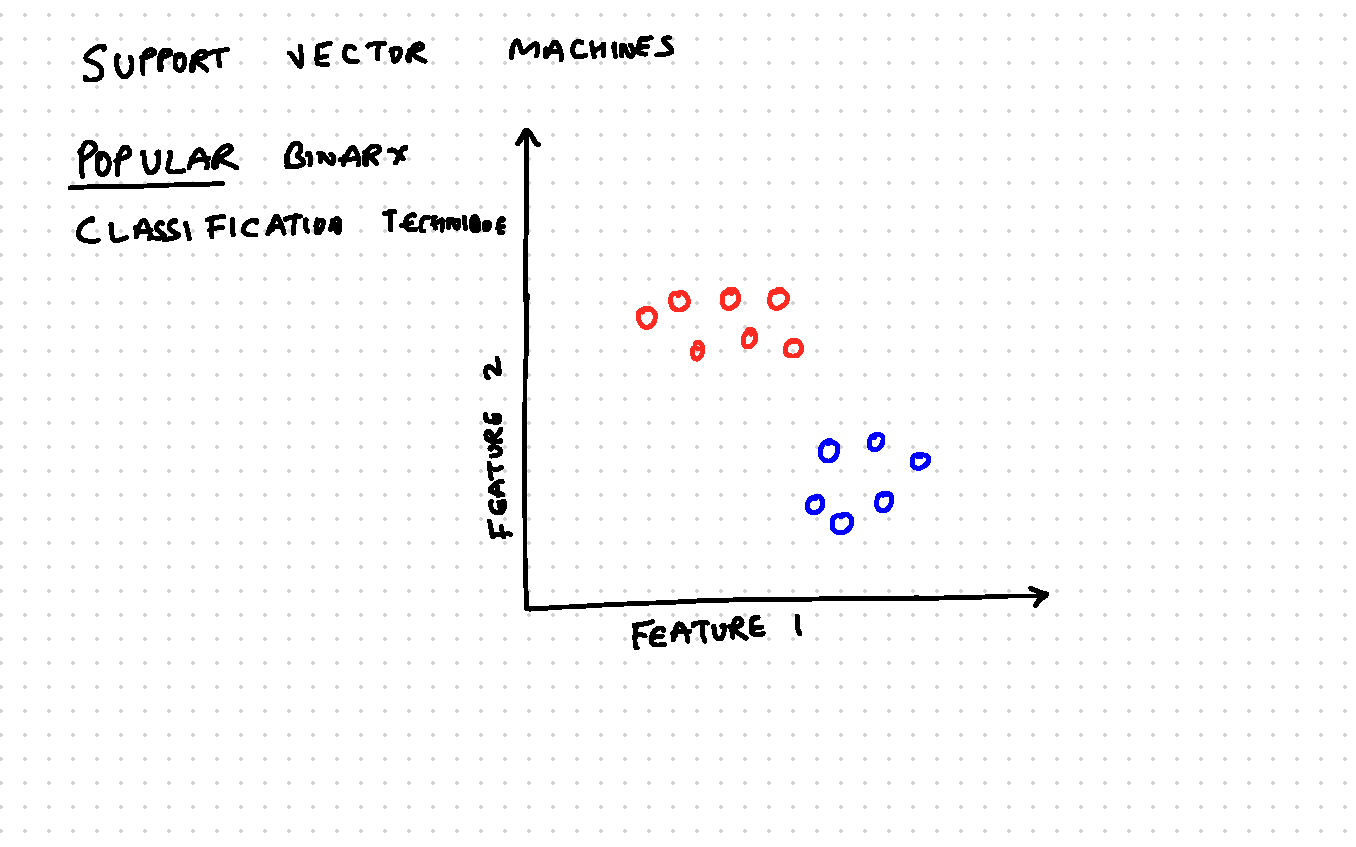
\includepdf[page=27]{../assets/svm/Svm-notes.pdf}
}


\begin{frame}{Revisiting the Simple Example}


\begin{equation*}
\begin{bmatrix}
x_{1} && y \\
1 && 1\\
2 && 1\\
-1 && -1\\
-2 && -1\\
\end{bmatrix}
\end{equation*}

\begin{align*}
L(\valpha) &= \sum_{i=1}^{4} \alpha_{i} - \frac{1}{2}\sum_{i=1}^{4}\sum_{j=1}^{4}\alpha_{i}\alpha_{j}y_{i}y_{j}x_i x_j \hspace{1cm}\alpha_{i} \geq 0 \\
&\sum \alpha_{i}y_{i} = 0 \hspace{1.5cm}
\alpha_{i}(y_{i}(w \cdot x_i + b) - 1) = 0
\end{align*}

\end{frame}

\begin{frame}{Pop Quiz \#4}
\begin{tcolorbox}[colback=blue!5!white,colframe=blue!75!black,title=Support Vector Challenge!]
In our 1D example with data points $\{(1,+1), (2,+1), (-1,-1), (-2,-1)\}$, which points will be the support vectors?

\pause
\textbf{Think:} Support vectors are the closest points to the decision boundary that actively constrain the solution.

\pause
\textbf{Answer:} Points $(1,+1)$ and $(-1,-1)$ are the support vectors!
\begin{itemize}
	\item These are closest to the decision boundary $x = 0$
	\item They satisfy $y_i(w \cdot x_i + b) = 1$ exactly
	\item Points $(2,+1)$ and $(-2,-1)$ are farther away $\Rightarrow$ $\alpha = 0$
\end{itemize}
\end{tcolorbox}
\end{frame}

\begin{frame}{Revisiting the Simple Example}
\begin{align*}
\begin{aligned}
\left.L(\alpha_{1},\alpha_{2},\alpha_{3},\alpha_{4}\right)=& \alpha_{1}+\alpha_{2}+\alpha_{3}+\alpha_{4} \\
&-\frac{1}{2}\left\{\alpha_{1} \alpha_{1}\times(1*1) \times(1 * 1)\right.\\
&\hspace{1cm} + \\
& \alpha_{1} \alpha_{2} \times(1*1) \times(1*2) \\
&\hspace{1cm}+\\
& \alpha_{1} \alpha_{3} \times(1*-1)\times(1*1)\\
& \hspace{1cm} ... \\
& \alpha_4\alpha_4 \times(-1*-1)\times(-2*-2)
\}
\end{aligned}
\end{align*}
How to Solve? $\Rightarrow$ Use the QP Solver!!
\end{frame}

\begin{frame}{Revisiting the Simple Example}
For the trivial example, \\
We know that only x = $\pm 1$ will take part in the constraint actively. Thus, $\alpha_2, \alpha_{4} = 0$ \\
\hspace{2cm} By symmetry, $\alpha_{1} = \alpha_{3} = \alpha $\text{ (say) }\\
\hspace{2cm} \& $\sum y_i\alpha_i = 0$
\begin{align*}
\begin{aligned}
\left.L(\alpha_{1},\alpha_{2},\alpha_{3},\alpha_{4}\right)=& 2\alpha \\
&-\frac{1}{2}\left\{\alpha^{2} (1)(-1)(1)(-1) \right. \\
&\hspace{1cm} + \alpha^{2} (-1)(1)(-1)(1) \\
&\hspace{1cm} + \alpha^{2} (1)(1)(1)(1) +  \alpha^{2} (-1)(-1)(-1)(-1) \\
\}\\
\end{aligned}
\end{align*}
\hspace{2cm} $\underset{\alpha}{Maximize} \hspace{3mm} 2\alpha - \frac{1}{2}(4\alpha^{2})$
\end{frame}

\begin{frame}{Revisiting the Simple Example}
\begin{align*}
\begin{aligned}
\frac{\partial}{\partial \alpha}\left(2 \alpha- 2\alpha^{2}\right)=0 & \Rightarrow 2-4 \alpha=0 \\
\Rightarrow \hspace{2mm}& \alpha=1/2\\
\end{aligned}\\
\therefore \alpha_{1}=1/2 \hspace{2mm} \alpha_{2}=0 ; \hspace{2mm} \alpha_{3}=1/2 \hspace{2mm} \alpha_{4}=0
\\
\vw=\sum_{i=1}^{N} \alpha_{i} y_{i} \bar{x}_{i} =1/2 \times 1 \times 1+0 \times 1 \times 2 \\
+ 1/2 \times -1 \times -1 + 0\times -1 \times -2 \\
 = 1/2 + 1/2 = 1
\end{align*}
\end{frame}

\begin{frame}{Revisiting the Simple Example}
\textbf{Finding b:}\\
For the support vectors we have, \\

$y_{i}(\vw \cdot \vx_{i}+b)-1=0$\\
or, $y_{i}$ $\left(\bar{w} \cdot \bar{x}_{1}+b\right)=1$\\
or, $y_{i}^{2}\left(\bar{w} \cdot \bar{x}_{i}+b\right)=y_{i}$\\
or, $\quad \bar{w}, \bar{x}_{i}+b=y_{i} \hspace{2mm}(\because y_{i}^{2} = 1)$\\
or, $b= y_i - w \cdot x_i$

In practice, $b=\frac{1}{N_{SV}} \sum_{i=1}^{N_{SV}}\left(y_{i}-\bar{w}\bar{x}_{i}\right)$

\end{frame}

\begin{frame}{Obtaining the Solution}
\begin{align*}
\begin{aligned}
b &=\frac{1}{2}\{(1-(1)(1))+(-1-(1)(-1))\\
&=\frac{1}{2}\{0+0\}=0 \\
&=0 \\
& \therefore w = 1 \hspace{2mm}\& \hspace{2mm} b = 0
\end{aligned}
\end{align*}
\end{frame}

\begin{frame}{Making Predictions}
\textbf{Making Predictions} \\
\hspace{2cm} $\hat{y}(x_i) = \operatorname{SIGN}(w \cdot x_i + b)$\\

For $x_{test} = 3$; $\hat{y}(3) = \operatorname{SIGN}(1 \times 3 + 0)$ = +ve class
\end{frame}

\begin{frame}{Making Predictions}
\begin{align*}
\begin{array}{l}
{\text {Alternatively, }} \\
{\qquad \begin{aligned}
\yhat(\vx_{\text{test}}) &=\sign(\vw \cdot \vx_{\text{test}}+b) \\
&=\sign \left(\sum_{j=1}^{N_{\text{SV}}} \alpha_{j} y_{j} \vx_{j} \cdot \vx_{\text{test}}+b\right)
\end{aligned}}
\end{array}
\end{align*}
\begin{align*}
\begin{aligned}
&\text{In our example,} \\
&\alpha_{1}=1/2 ; \alpha_{2}=0 ; \quad \alpha_{3}=1/2 ; \alpha_{4}=0\\
&\yhat(3) =\sign\left(\frac{1}{2} \times 1 \times (1 \times 3)+0+\frac{1}{2} \times (-1) \times (-1 \times 3)+0\right)\\
&=\sign \left(\frac{6}{2}\right)=\sign(3)=+1
\end{aligned}
\end{align*}

\end{frame}

\begin{frame}{Pop Quiz \#5}
\begin{tcolorbox}[colback=blue!5!white,colframe=blue!75!black,title=Prediction Power!]
We found our SVM solution: $w = 1, b = 0$. Let's test it!

What will our SVM predict for the test point $x_{\text{test}} = -0.5$?

\pause
\textbf{Method 1:} Direct: $\yhat(-0.5) = \sign(1 \times (-0.5) + 0) = \sign(-0.5) = -1$

\pause  
\textbf{Method 2:} Using support vectors:
$\yhat(-0.5) = \sign(\frac{1}{2} \times 1 \times 1 \times (-0.5) + \frac{1}{2} \times (-1) \times (-1) \times (-0.5))$
$ = \sign(-0.5) = -1$ (Correct!)
\end{tcolorbox}
\end{frame}

\section{Kernel Methods}

{
	\setbeamercolor{background canvas}{bg=}
	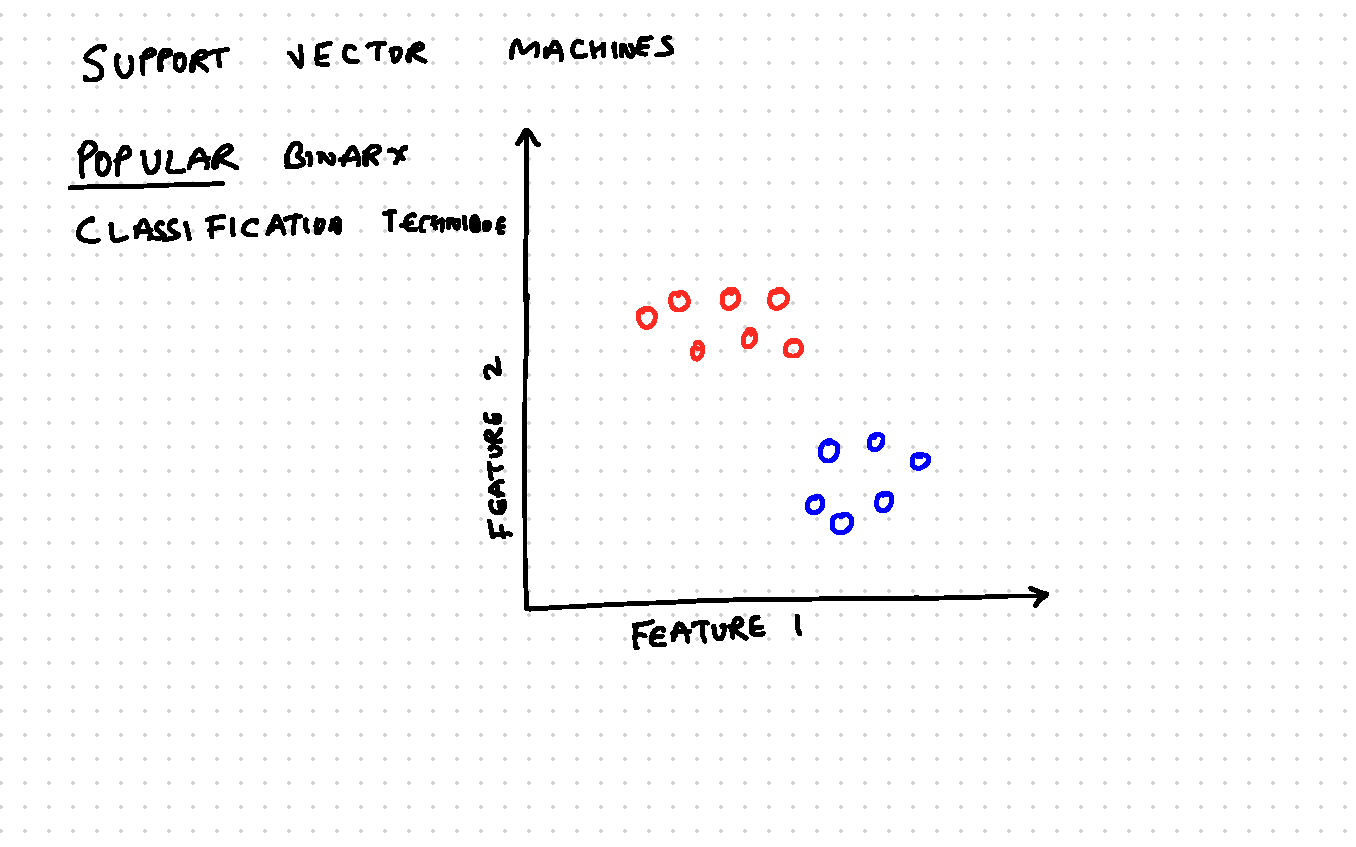
\includepdf[page=35-35]{../assets/svm/Svm-notes.pdf}
}

\begin{frame}{Non-Linearly Separable Data}
	\begin{itemize}
		\item Data is not linearly separable in $\mathbb{R}^d$.
		\item Can we still use SVM?
		\item Yes! Project data to a higher dimensional space.
	\end{itemize}
	\end{frame}

\subsection{Kernel Motivation}

{
	\setbeamercolor{background canvas}{bg=}
	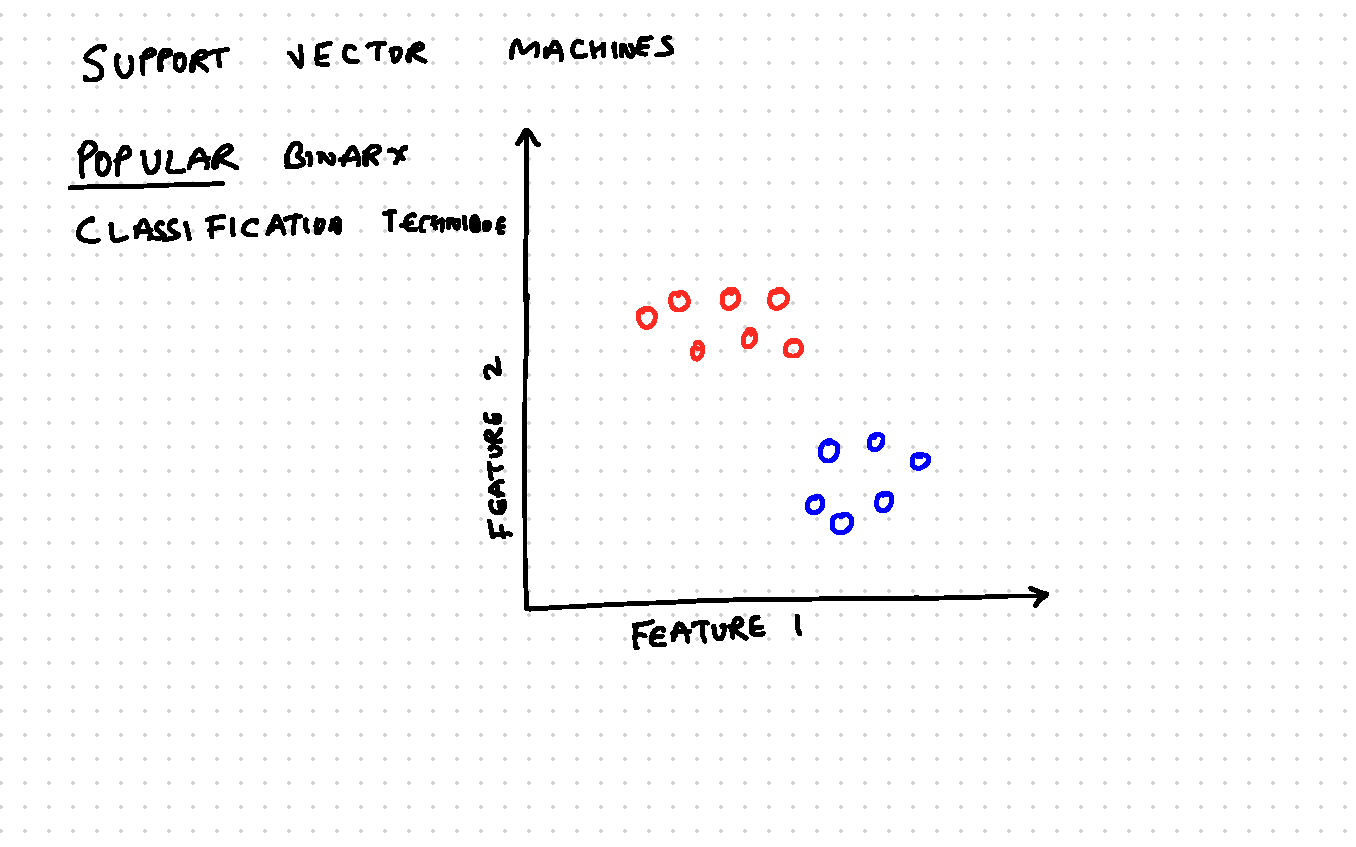
\includepdf[page=36-41]{../assets/svm/Svm-notes.pdf}
}

\begin{frame}{Projection/Transformation Function}
	        $\phi : \mathbb{R}^{d} \rightarrow \mathbb{R}^{D}$
	    
	    where, $d$ = original dimension \\
	    \hspace{1cm} $D$ = new dimension \\
	    In our example:\\
	    \hspace{1cm} $d = 1; D = 2$ 
	\end{frame}
	\begin{frame}{From Linear to Kernel SVM}
	    Linear SVM:\\
	    \hspace{1cm} Maximize\\
	    \begin{equation*}
	        L(\alpha) = \sum_{i=1}^{N}\alpha_{i} - \frac{1}{2}\sum_{i=1}^{N}\sum_{j=1}^{N}\alpha_{i}\alpha_{j}y_{i}y_{j}\vx_{i} \cdot \vx_{j}
	    \end{equation*}
	    \hspace{1cm} such that constriants are satisfied.\\
	   \hspace{5cm} $\downarrow$\\
	   \hspace{3.8cm} Transformation ($\phi$)\\
	   \hspace{5cm} $\downarrow$\\
	   \begin{equation*}
	       L(\alpha) = \sum_{i=1}^{N}\alpha_{i} - \frac{1}{2}\sum_{i=1}^{N}\sum_{j=1}^{N}\alpha_{i}\alpha_{j}y_{i}y_{j}\phi(\vx_{i}) \cdot \phi(\vx_{j})
	   \end{equation*}
	\end{frame}


	\begin{frame}{Steps}
	    \begin{enumerate}
	        \item Compute $\phi(\vx)$ for each point \\
	        \begin{equation*}
	            \phi: \mathbb{R}^{d} \rightarrow \mathbb{R}^{D}
	        \end{equation*}
	        \item Compute dot products over $\mathbb{R}^{D}$ space
	    \end{enumerate}
	    \hspace{0.1cm} Q. If $D >> d$ \\
	    \hspace{0.6cm} Both steps are expensive!
	\end{frame}
	\begin{frame}{The Kernel Trick}
	\textbf{Brilliant idea:} Can we compute $K(\vx_{i}, \vx_{j})$ such that:
	$$K(\vx_{i}, \vx_{j}) = \phi(\vx_{i}) \cdot \phi(\vx_{j})$$
	
	\textbf{Without explicitly computing $\phi$!}
	
	\begin{itemize}
		\item $K(\vx_{i}, \vx_{j})$: Simple function in original space
		\item $\phi(\vx_{i}) \cdot \phi(\vx_{j})$: Complex dot product in high-dimensional space
	\end{itemize}
	
	\textbf{Result:} Get non-linear classification power without computational cost!
	\end{frame}

\subsection{Kernel Examples}

	{
	\setbeamercolor{background canvas}{bg=}
	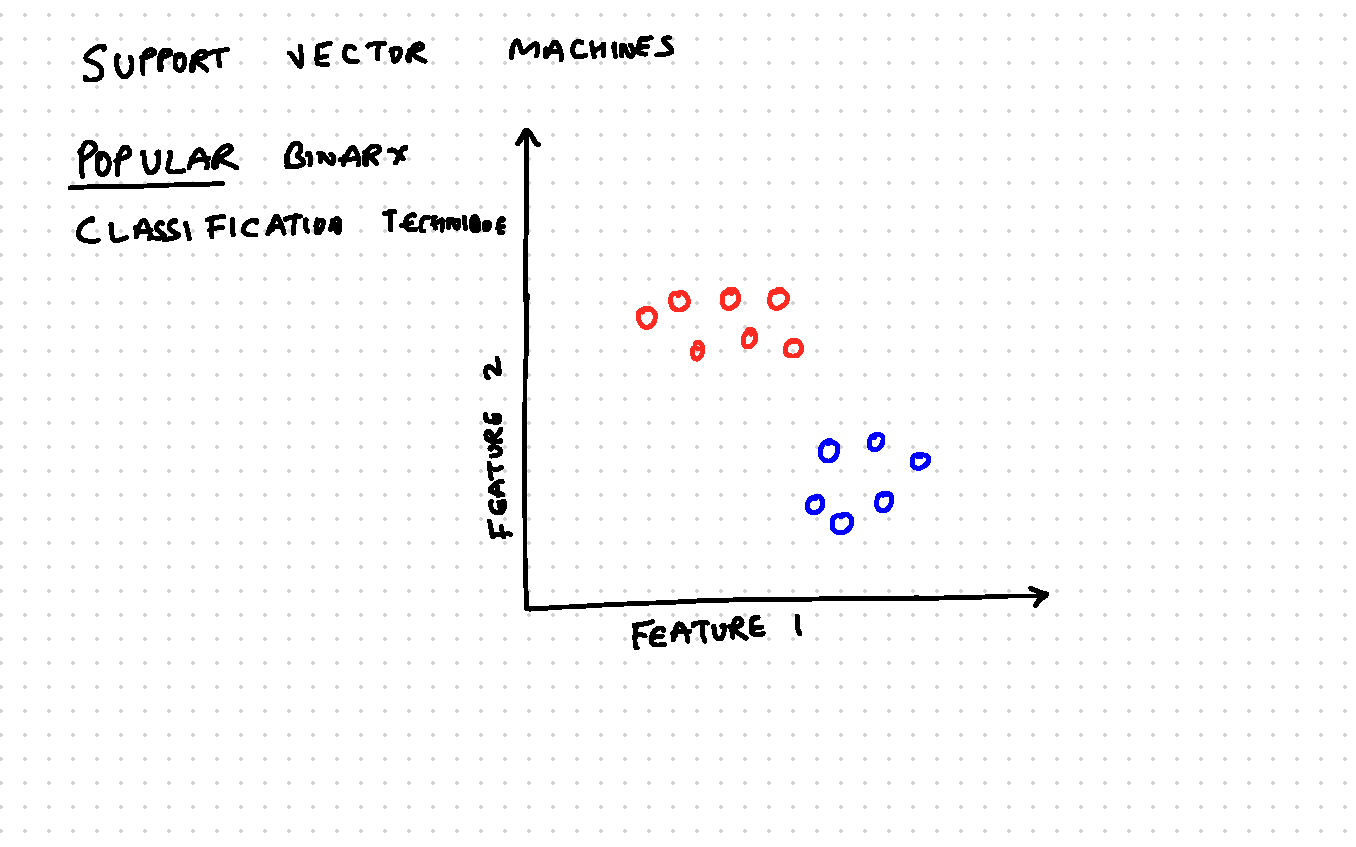
\includepdf[page=41-47]{../assets/svm/Svm-notes.pdf}
}

\begin{frame}{Kernel Trick}
	   Q) Why did we use dual form? \\
	   \hspace{0.5cm} Kernels again!! \\
	   \vspace{1cm}
	   Primal form doesn't allow for the kernel trick \\
	   $K(\vx_{1}, \vx_{2})$ in dual and compute $\phi(\vx)$ and then dot product in $D$ dimensions
	\end{frame}
	\begin{frame}{Gram Matrix: (Positive Semi-Definite)}
	$K(\vx_{i}, \vx_{j}) = (1 + \vx_{i} \cdot \vx_{j})^{2}$ \\
	$$
	\begin{matrix}
	& x_{1} & x_{2} & x_{3} & x_{4} & x_{5} & x_{6} & x_{7} \\
	x_{1} & 24 & 8 & 0 & 0 & 8 & 24 & 48 \\
	x_{2} & 8 & 1 & 0 & -1 & 0 & \ldots & \\
	x_{3} & 0 & \ldots & \ldots & \ldots & \ldots & \ldots & \ldots \\
	x_{4} & 0 & & & & & & \\
	x_{5} & 8 & & & & & & \\
	x_{6} & 24 & & & & & & \\
	x_{7} & 48 & & & & & & \\
	\end{matrix}
	$$
	\end{frame}

	\begin{frame}{Common Kernel Functions}
	\textbf{Most frequently used kernels:}
	    \begin{enumerate}
	        \item \textbf{Linear:} $K(\vx_{1}, \vx_{2}) = \vx_{1} \cdot \vx_{2}$
	        \item \textbf{Polynomial:} $K(\vx_{1}, \vx_{2}) = (c + \vx_{1} \cdot \vx_{2})^{d}$
	        \item \textbf{RBF (Gaussian):} $K(\vx_{1}, \vx_{2}) = \exp(-\gamma\norm{\vx_{1} - \vx_{2}}^{2})$
	    \end{enumerate}
	    
	    \vspace{0.5cm}
	    \textbf{Parameters:}
	    \begin{itemize}
	    	\item $c$: constant term, $d$: degree (polynomial)
	    	\item $\gamma$: bandwidth parameter (RBF)
	    \end{itemize}
	\end{frame}
	\begin{frame}{Kernel Example: Polynomial Kernel}
	    \textbf{Question:} For $\vx = \begin{bmatrix}x_{1} \\ x_{2} \end{bmatrix}$, what is the feature space for $K(\vx, \vz) = (1 + \vx \cdot \vz)^{3}$?
	    
	    \textbf{Given:} $\vx \in \Real^{2}$, find dimension of $\phi(\vx)$
	    
	    \textbf{Expansion:}
	    \begin{align*}
	        K(\vx, \vz) &= (1 + x_{1}z_{1} + x_{2}z_{2})^{3} \\
	        &= \text{all terms of degree } \leq 3 \\
	        &= \phi(\vx) \cdot \phi(\vz)
	    \end{align*}
	    
	    \textbf{Feature map:} $\phi(\vx) = [1, \sqrt{3}x_1, \sqrt{3}x_2, \sqrt{3}x_1^2, \sqrt{3}x_2^2, \sqrt{6}x_1x_2, x_1^3, x_2^3, \sqrt{3}x_1^2x_2, \sqrt{3}x_1x_2^2]$
	    
	    \textbf{Answer:} $\phi(\vx) \in \Real^{10}$
	\end{frame}
	\begin{frame}{RBF Kernel: Infinite Dimensions}
	    \textbf{Question:} What is the dimensionality of RBF kernel feature space?
	    
	    \textbf{RBF Kernel:}
	    \begin{align*}
	        K(x, z) &= \exp(-\gamma\norm{x - z}^{2})\\
	        &= \exp(-\gamma(x - z)^{2})
	    \end{align*}
	    
	    \textbf{Key insight:} Using Taylor series expansion
	    $$\exp(\alpha) = \sum_{n=0}^{\infty}\frac{\alpha^{n}}{n!} = 1 + \alpha + \frac{\alpha^2}{2!} + \frac{\alpha^3}{3!} + \cdots$$
	    
	    \textbf{Result:} RBF kernel corresponds to $\infty$-dimensional feature space!
	    
	    \textbf{Amazing:} Infinite-dimensional classification with finite computation!
	\end{frame}
	
	\begin{frame}{Does RBF Involve Dot Product in Lower-Dimensional Space?}
	\textbf{Question:} Can we see the original dot product in RBF kernel?
	
	Assuming $\vx$ is a one-dimensional vector, we can rewrite the RBF kernel as:
	$$K(x, z) = \exp(-\gamma\norm{x-z}^{2}) = \exp(-\gamma(x-z)^{2})$$
	
	\pause
	\textbf{Expanding the squared term:}
	$$(x - z)^{2} = x^{2} - 2xz + z^{2}$$
	
	\pause
	\textbf{Substituting back into the RBF kernel:}
	\begin{align*}
	K(x, z) &= \exp(-\gamma(x^{2}-2xz+z^{2})) \\
	&= \exp(-\gamma x^{2}) \cdot \exp(2\gamma xz) \cdot \exp(-\gamma z^{2})
	\end{align*}
	
	\textbf{Key insight:} The middle term $\exp(2\gamma xz)$ contains the dot product $xz$ from the original space!
	\end{frame}
	
	\begin{frame}{SVM: Parametric vs Non-Parametric}
	    \textbf{Question:} Is SVM parametric or non-parametric?
	    
	    \pause
	    \textbf{Answer:} It depends on the kernel!
	    
	    \begin{itemize}
	    	\item \textbf{Parametric:} Linear and polynomial kernels
	    		\begin{itemize}
	    			\item Fixed functional form
	    			\item Number of parameters independent of training data size
	    		\end{itemize}
	    	\item \textbf{Non-parametric:} RBF kernel
	    		\begin{itemize}
	    			\item Model complexity grows with data
	    			\item Uses all support vectors for prediction
	    		\end{itemize}
	    \end{itemize}
	\end{frame}
	\begin{frame}{RBF is Non-Parametric}
	    \begin{align*}
	        \yhat(\vx_{\text{test}}) &= \sign(\vw \cdot \vx_{\text{test}} + b) \\
	        &= \sign(\sum_{j=1}^{N_{\text{SV}}}\alpha_{j}y_{j}\vx_{j} \cdot \vx_{\text{test}} + b)\\
	        \yhat(\vx_{\text{test}}) &= \sign(\sum_{j=1}^{N}\alpha_{j}y_{j} K(\vx_{j}, \vx_{\text{test}}) + b)
	    \end{align*}
	    $\alpha_{j} = 0$ where $j \neq$ S.V.
	\end{frame}

	\begin{frame}{Interpretation of RBF}
		\begin{itemize}[<+->]
			\item $\yhat(\vx) = \sign(\sum \alpha_{i}y_{i}\exp(-\norm{\vx - \vx_{i}}^{2}) + b)$
			\item $-\norm{\vx - \vx_{i}}^{2}$ corresponds to radial term
			\item $\sum \alpha_{i}y_{i}$ is the activation component
			\item $\exp(-\norm{\vx - \vx_{i}}^{2})$ is the basis component
		\end{itemize}
	    
	    
	\end{frame}

\subsection{Kernel Properties}

		{
	\setbeamercolor{background canvas}{bg=}
	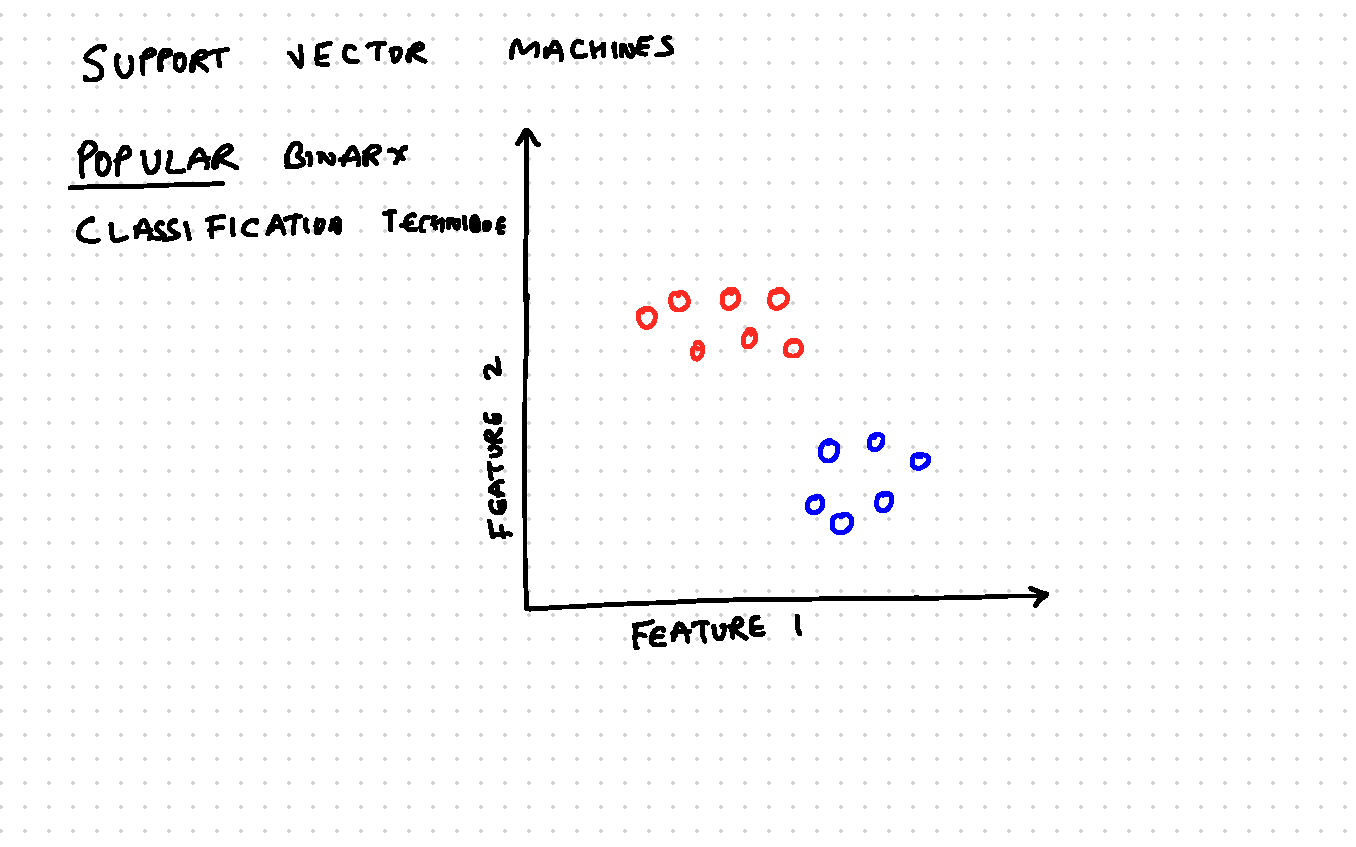
\includepdf[page=48-49]{../assets/svm/Svm-notes.pdf}
}

\section{Summary}

\begin{frame}{Key Takeaways}
\begin{itemize}
	\item \textbf{Goal:} SVM finds optimal separating hyperplane by maximizing margin
	\item \textbf{Math:} Dual formulation enables kernel trick
	\item \textbf{Power:} Kernels enable non-linear classification without explicit mapping
	\item \textbf{Popular kernels:} Linear, Polynomial, RBF (Gaussian)
	\item \textbf{Remarkable:} RBF kernel $\leftrightarrow$ infinite-dimensional space
	\item \textbf{Flexibility:} Parametric (linear/poly) or non-parametric (RBF)
	\item \textbf{Efficiency:} Only support vectors matter for prediction
\end{itemize}
\end{frame}

\begin{frame}{Next Steps}
\begin{itemize}
	\item Soft-margin SVM for non-separable data
	\item Hyperparameter tuning (C, $\gamma$)
	\item Multi-class SVM extensions
	\item Computational considerations and optimization
	\item Comparison with other classifiers
\end{itemize}
\end{frame}

\end{document}
